\documentclass{article}
\usepackage[utf8]{inputenc}
\usepackage[hidelinks]{hyperref}
\usepackage[a4paper]{geometry}
\usepackage{amssymb}
\usepackage{graphicx}
\usepackage{fancyhdr}
\usepackage{titlesec}

\titleformat*{\section}{\LARGE\bfseries}
\titleformat*{\subsection}{\Large\bfseries}

\pagestyle{fancy}

\lhead{\leftmark}
\rhead{Page \thepage}
\cfoot{Ojas Karanjkar 210070040}
\renewcommand{\footrulewidth}{1pt}

\begin{document}

\begin{titlepage}
\begin{center}
    \vspace*{\fill}
\includegraphics[scale=0.4]{iitb.png}\\
[4 cm]
    \rule{12.5cm}{0.75mm}\\
    \huge{\bfseries Filter Design Assignment-I}
    \rule{12.5cm}{0.75mm}\\
    [0.5cm]
   {\textbf {EE338 - 2023 \\
    Chebyshev Bandpass Filter Review Report}}\\
    [2.5cm]
\end{center}
\begin{flushleft}
   {\huge
    Ojas Karanjkar \\
    210070040 \\
     \\}
    \end{flushleft}
\end{titlepage}
\tableofcontents
\thispagestyle{empty}
\clearpage
\pagenumbering{arabic}

\newpage

\section{Student Details}
\begin{itemize}
    \item Name : Ojas Karanjkar
    \item Roll No: 210070040
    \item Filter number assigned: 103
\end{itemize}

\section{Chebyshev Bandpass Filter Details}
\subsection{Un-normailzed Discrete time specifications}

\begin{itemize}
    \item \begin{enumerate}
                \item m = 23
                \item q(m) = [2.3] = 2
                \item r(m) = 23 - 10*2 = 3
                \item BL(m) = 20 + 3*2 + 11*3 = 59
                \item BH(m) = 59 + 75 = 134
            \end{enumerate}

    \item Passband = $59$ kHz to $134$ kHz.
    \item Transition Band Width = $5$ kHz.
    \item Stopband = $0$ to $54$ kHz and $139$ to $300$ kHz.
    \item Tolerance = 0.15.
    \item Nature of Passband = Equiripple.
    \item Nature of Stopband = Monotonic.
\end{itemize}


\begin

\subsection{Normailzed discrete filter specifications}
Sampling frequency = $600 kHz$\\
\begin{equation}
    \omega = \frac{\Omega * 2\pi}{\Omega _{sampling}}\\
\end{equation}

\begin{itemize}
    \item Passband = $0.1967\pi$ to $0.4467\pi$ .
    \item Transition Band Width = $0.0167\pi$ .
    \item Stopband = $0$ to $0.18$  and $0.4633\pi$ to $\pi$ .
    \item Tolerance = 0.15.
    \item Nature of Passband = Equiripple.
    \item Nature of Stopband = Monotonic.
\end{itemize}


\subsection{Converting to Analog Low-pass filter}
We have the following transformation for converting into analog low-pass filter:\\
\begin{equation}
    \Omega = tan(\frac{\omega}{2})\\
\end{equation}

Using the above Bilinear Transformation, the passband and stopband specifications are updated as follows:\\

\begin{itemize}
    \item Passband = $0.3191$ to $0.8451$ .
    \item Transition Band = $0.2905$ to $0.3191$ and $0.8451$ to $0.8910$ .
    \item Stopband = $0$ to $0.2905$  and $0.8910$ to $\infty$ .
    \item Tolerance = 0.15.
    \item Nature of Passband = Equiripple.
    \item Nature of Stopband = Monotonic.
\end{itemize}

\subsection{Frequency Transformation for Band-Stop Filter}
The frequency transformation for converting a bandpass filter to low pass filter are as follows:\\

\begin{equation}
    \Omega _{L} = \frac{\Omega _{0}^{2} - \Omega^{2}}{B\Omega}  \\
\end{equation}

\begin{equation}
    B = \Omega _{p2} - \Omega _{p1} \\
\end{equation}

\begin{equation}
    \Omega _{0} = \sqrt{\Omega _{p1}\Omega _{p2}}\\
\end{equation}

According to the above transformation, we can tabulate the updated value of passband and stopband edges:\\

\begin{table}[h]
    \centering
    \begin{tabular}{|c|c|}
        \hline
       $\Omega$ & $\Omega _{L}$\\
       \hline
       $0^+$  & $-\infty$   \\
       \hline
       $0.3191 (\Omega_{p1})$  & $-1$   \\
       \hline
        $0.2905 (\Omega_{s1})$  & $-1.2127$   \\
       \hline
       $0.5193 (\Omega_{0})$  & $0$   \\
       \hline
       $0.8910 (\Omega_{s2})$  & $1.1185$   \\
       \hline
       $0.8451 (\Omega_{p2})$  & $1$   \\
       \hline
       $\infty$  & $\infty$   \\
       \hline
    \end{tabular}
\end{table}

\begin{itemize}
    \item Passband edge = 1 ($\Omega_{lp}$)
    \item Stopband edge = 1.1185 ($\Omega_{ls}$)
    \item Tolerance = 0.15.
    \item Nature of Passband = Equiripple.
    \item Nature of Stopband = Monotonic.
\end{itemize}

\subsection{Analog Lowpass Transfer Function}
 Tolerance = 0.15\\

 \begin{equation}
     D_{1} = \frac{1}{(1-\delta)^2} - 1 = 0.3844\\
 \end{equation}

\begin{equation}
    D_{2} = \frac{1}{\delta^2} - 1 = 43.44 \\
\end{equation}

We take $\epsilon$ to be equal to $\sqrt{D_{1}}$ and calculate N as follows:

\begin{equation}
    N \geq \lceil \frac{cosh^{-1}\sqrt{\frac{D_{2}}{D_{1}}}}{cosh^-1\frac{\Omega_{Ls}}{\Omega_{Lp}}} \rceil \\
\end{equation}

Substituting the values in above equation gives N to be equal to $7$.\\

 \subsubsection{Finding Poles of the transfer function}

 Poles can be found using the following expression:\\

 \begin{equation}
     1 + 0.3841cosh^{2}(7cosh^{-1}()\frac{s}{\iota}) = 0
 \end{equation}

 Upon solving the above equation we get the following value of poles in open left half complex plane:\\

\begin{center}
p1 =$ -0.1625 + \iota 0.4409$\\
p2 = $-0.1625 - \iota 0.4409$\\
p3 = $-0.0.401 + \iota 0.9907$\\
p4 = $-0.0.401 - \iota 0.9907$\\
p5 = $-0.1125 + \iota 0.7945$ \\
p6 = $-0.1125 - \iota 0.7945$ \\
p7 = $-0.1804$\\

\end{center}
The plot of the poles of the magnitude response of the Analog Lowpass filter plotted in python is as follows:-

\newpage
\begin{center}
     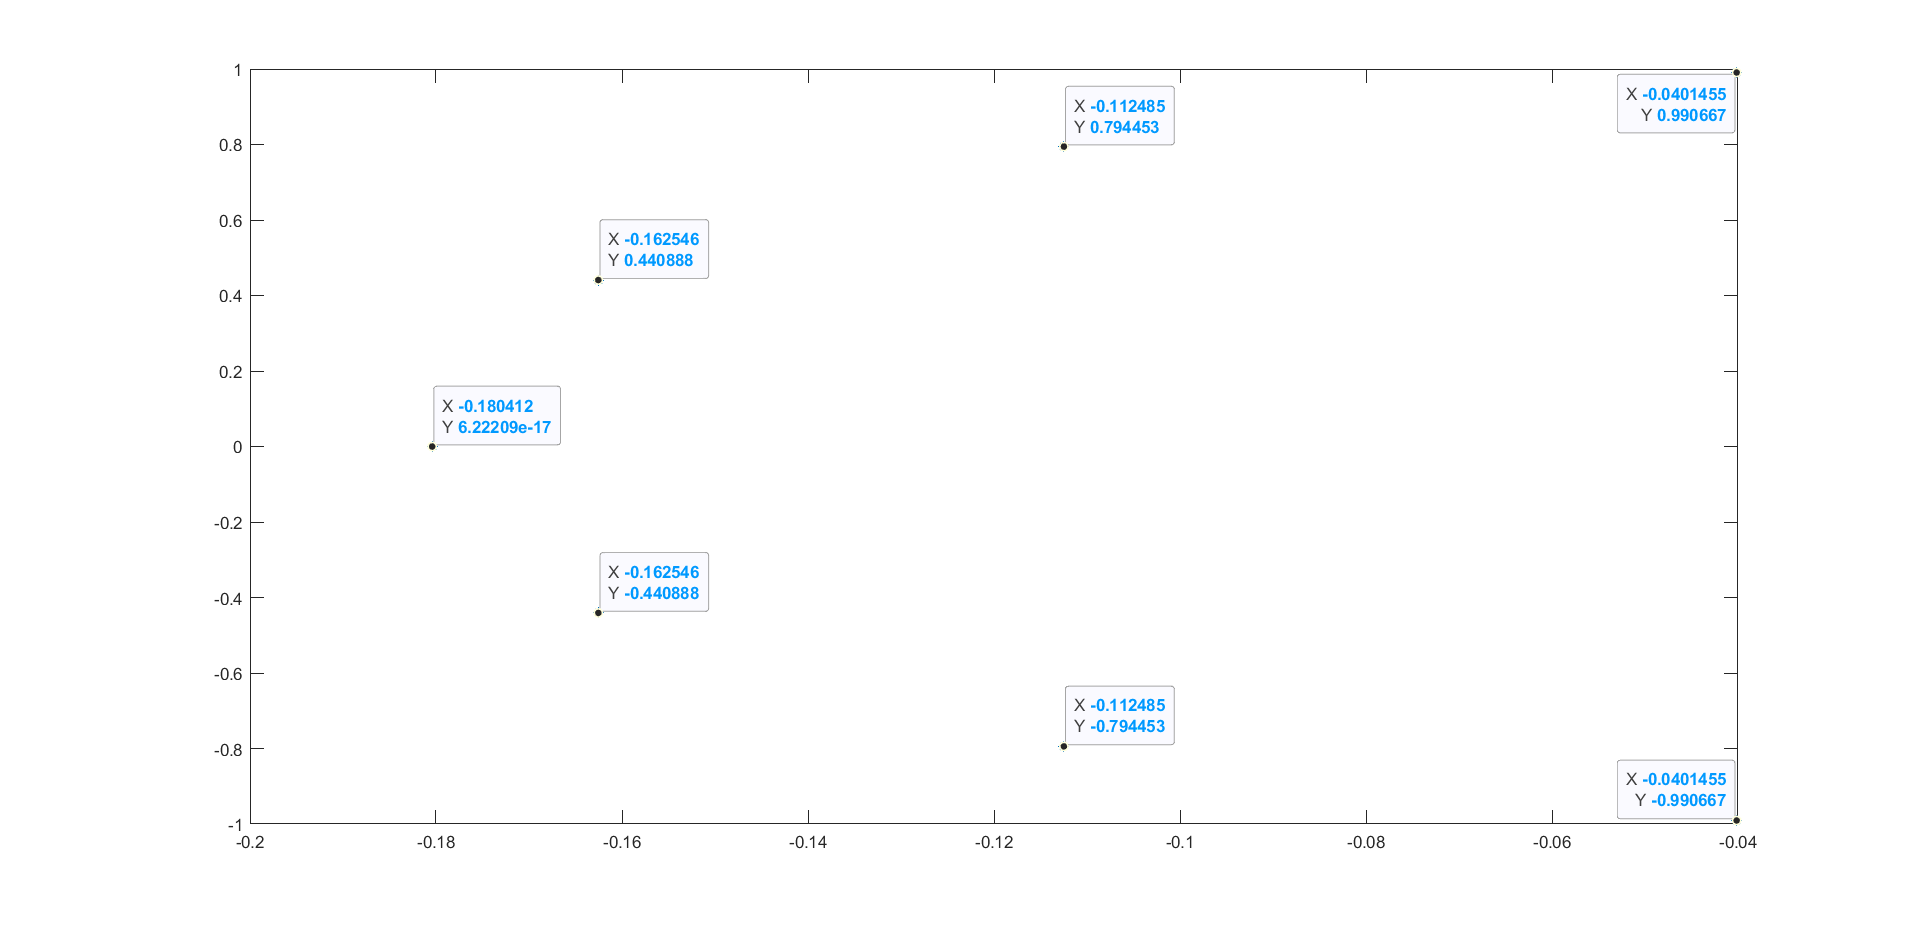
\includegraphics[scale = 0.25]{poles.png}\\
    \caption{Poles of Magnitude response}\\
\end{center}
   
The Transfer Function of the Analog Lowpass Filter:\\

\[H_{analog,LPF}(s_{L}) = \frac{(-1)^{N}p_{1}p_{2}p_{3}p_{4}p_{5}p_{6}p_{7}}{\Pi_{i=1}^{7} (s-p_{i})} \]\\

 \subsection{Analog Bandstop Transfer Function}

Now we need to transform the Analog Lowpass filter back to Analog Bandpass filter using the same transformation we used earlier.
\[s_{L} = \frac{\Omega_{0}^2 + s^2}{Bs}\]
Thus
\[s_{L} = \frac{0.2697 + s^2}{0.5259s}\]

Substituting this value of $s_{L}$ into the above Analog Lowpass Filter Tranfer Function to get the Analog Bandpass Filter Tranfer function i.e \textbf{$H_{analog,BPF}(s)$}. Numerator and Denominator coefficients are as follows:



\begin{table}[H]
  \begin{minipage}{.5\linewidth}
    \centering
    \begin{tabular}{ |c|c| }
      \hline
      {Powers of s \\ in Numerator} & \makecell{Coefficients} \\
      \midrule
      \hline
      $s^{7}$ & 0.2806\\
      \hline
      \bottomrule
    \end{tabular}
  \end{minipage}%
  \begin{minipage}{.5\linewidth}
    \centering
    \begin{tabular}{ |c|c| }
      \hline
      {Powers of s \\ in Denominator} & \makecell{Coefficients} \\
      \midrule
      \hline
      $s^{14}$ & 1 \\
      \hline
      $s^{13}$ & 0.4264 \\
      \hline
      $s^{12}$ & 2.4628 \\
      \hline
      $s^{11}$ & 0.8688 \\
      \hline
      $s^{10}$ & 2.3978 \\
      \hline
      $s^{9}$ & 0.6767\\
      \hline
      $s^{8}$ & 1.1857 \\
      \hline
      $s^{7}$ & 0.2556 \\
      \hline
      $s^{6}$ & 0.3198 \\
      \hline
      $s^{5}$ & 0.0492 \\
      \hline
      $s^{4}$ & 0.0470 \\
      \hline
      $s^{3}$ & 0.0046 \\
      \hline
      $s^{2}$ & 0.0035\\
      \hline
      $s^{1}$ & 0.0002 \\
      \hline
      $s^{0}$ & 0.0001 \\
      \hline
      \bottomrule
    \end{tabular}
  \end{minipage}
\end{table}

 
\begin{table}[H]
  \begin{minipage}{.5\linewidth}
    \centering
    \begin{tabular}{ |c|c| }
    \hline
      {Powers of z \\ in Denominator} & \makecell{Coefficients} \\
      \hline
      $z^{-14}$ & 1 \\
      \hline
      $z^{-13}$ & -7.1112 \\
      \hline
      $z^{-12}$ & 27.3168 \\
      \hline
      $z^{-11}$ & -71.8033 \\
      \hline
      $z^{-10}$ & 142.5073 \\
      \hline
      $z^{-9}$ & -224.0436 \\
      \hline
      $z^{-8}$ & 286.1419 \\
      \hline
      $z^{-7}$ & -300.7474 \\
      \hline
      $z^{-6}$ & 261.3445 \\
      \hline
      $z^{-5}$ & -186.8610 \\
      \hline
      $z^{-4}$ & 108.5512 \\
      \hline
      $z^{-3}$ & -49.8857 \\
      \hline
      $z^{-2}$ & 17.3512\\
      \hline
      $z^{-1}$ & -4.3110 \\
      \hline
      $z^{0}$ & 0.5295\\
      \hline
      \bottomrule
    \end{tabular}
  \end{minipage}%
  \begin{minipage}{.5\linewidth}
    \centering
    \begin{tabular}{ |c|c| }
    \hline
      Powers of s \\ in Numerator & Coefficients \\
      \hline
      $z^{-12}$ & -0.0002\\
      \hline
      $z^{-10}$ & 0.0006 \\
      \hline
      $z^{-8}$ & -0.0010 \\
      \hline
      $z^{-6}$ & 0.0010 \\
      \hline
      $z^{-4}$ & -0.0006 \\
      \hline
      $z^{-2}$ & 0.002\\
      \hline
      \bottomrule
    \end{tabular}
  \end{minipage}
\end{table}

\newpage
\subsection{Peer Review}
I have reviewed the chebyschev filter design of Kushal Gajbe, Roll No. 210070048. I have gone through his matlab code for chebyshev bandpass filter. I have observed that, he made functions for calculating the values of the parameters for the filter and transformation as well. I have checked the correctness of those functions and can say that the values he got are correct.I have cross checked the value of poles and those are correct as well. Finally, he has correctly written the transfer functions and the magnitude and phase response plots are correct as well. Hence, I certify the chebyschev bandpass filter, that Kushal Gajbe has designed to be correct.

\end{document}
